\section{Frontend}
\label{sec:frontend}

\subsection{Location Awareness}

To provide the possibility to find nearby venues and friends the application needs to be aware of the location of the user and his friends. A background service, which tracks the location of the users has been implemented to achieve this. The location data is the provided to the search, the map and the server.

\subsubsection{LocationService}
The LocationService is a simple background service which is started at the start of the app and it is stopped, when the MainActivity is destoryed. The main functionality is to controll the LocationTracker which actually tracks the location.

\subsubsection{LocationTracker}
The LocationTracker is implemented as an LocationListener. The GooglePlayService API is used to obtain the location every intervall. The intervall is parameterized.

There are two different modes to guarantee a balance between power usage and accuracy. If the user is going to send a searchrequest by starting to search for a venue, the priority of the GoogleAPI client is set on high accuracy, otherwise and after the search, the mode is set on balance between accuracy and power usage.Moreover there is a check if the necessary Permissions are provided or not. On every change of the location, the location is send as a LocationEvent over the EventBus. 

\subsection{Communication via greenrobot.org/EventBus}

To communicate between the service and the acticity and fragements the greenrobot.org/EventBus is used. There are two different events which are posted on the bus and three different cases:


\begin{figure}[htbp]
	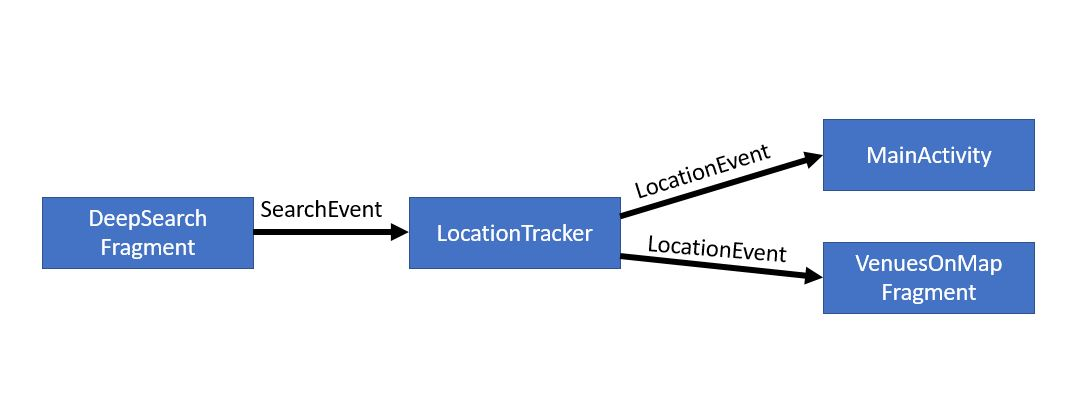
\includegraphics[width=0.8\textwidth]{images/eventBus.jpg}
	\centering
	\caption[]{EventBus Graph, schematically shows who sends which kind of an event and who receives it}
	\label{fig:eventbus}
\end{figure} 


\begin{itemize}
\item The LocationTracker subscribes on it to receive the SearchEvent, which tells it to change the accuracy
\item The SearchEvent is posted by the DeepSearchFragement everytime its view is created
\item The LocationTracker posts a LocationEvent on the EventBus, which contains the Location and is received by the MainActivity and the VenueOnMapFragment
\item The MainActivity receives the LocationEvent, stores it locally and sends it every 10 seconds (parameterized) to the server, to update the users position data
\item The VenueOnMapFragment receives the LocationEvent to update the Location of the user on the map and also the location of his friends if the user is logged in
\end{itemize}

\subsection{The Map}
The map is used as a function to show the user graphically where he and his nearby friends are and also the searched venues. The functionality of the map in inside the VenuesOnMapFragment, which is part of the MainActivity. The map itself is provided by GoogleMaps.

There are three different kinds of markers shown on the map. If the user clicks on any marker, a button shows up, which allows him to change to GoogleMaps and gets the route to the chosen marker. 

\subsubsection{Marker: Venue}
The venue markers locate the search results on the map. They differ in color, depending on the rating of the venue. Those colors are with the following more or less obvious order:

\begin{itemize}
\item grey: No rating available / no rating yet
\item red: rating between 0 and 1
\item orange: rating between 1 and 2
\item yellow: rating between 2 and 3
\item lime: rating between 3 and 4
\item green: rating between 4 and 5
\end{itemize}

If the user clicks on one of the markers an infoWindow shows up, which shows on image and tells the name, the exact rating and if it is open right now or not. With a click on the infoWindow the user is redirected to the VenueDetails, where he can find more additional information about the venue.

\subsection{Marker: Friend}
The friend markers locate the friends of the user, if he is logged in and has nearby (within TODO) friends. The marker of the friends is similar to the marker of the user, except it is green.
The Position of his nearby friends are updated everytime, the location of the user changes. 

If the user clicks on on of his friends marker, an infoWindow shows up with the avatar and name and if given, also the city and age. With a click on the infoWindow the user gets to the profile of his friend.

\subsection{Marker: User}
The User marker locate the user on the map. If the user clicks on himself, a infoWindow shows up. If the user is not logged in, it shows the default infoWindow with the default avatar. If the user is logged in, it shows his own avatar and additonal info. 

If he clicks on the infoWindow he is redirected to his own profile.

 



